\chapter{Abschlussaufgabe Mean Shift}
Mean Shift ist ein parameterfreier Clusteralgorithmus, bei welchem Punkte Clustern zugeordnet werden. Mean Shift findet Anwendung beim Clustering,
Tracking und bei Bildfiltern.\\
Nach einer Einführung in die Funktionsweise des Algorithmus wird auf die sequentielle und parallele Implementation eingegangen.
Abschließend werden Benchmarks zum Speedup und Laufzeit der Implementation betrachtet.\\
\vspace{-10pt}
\begin{figure}[H]
	\centering
	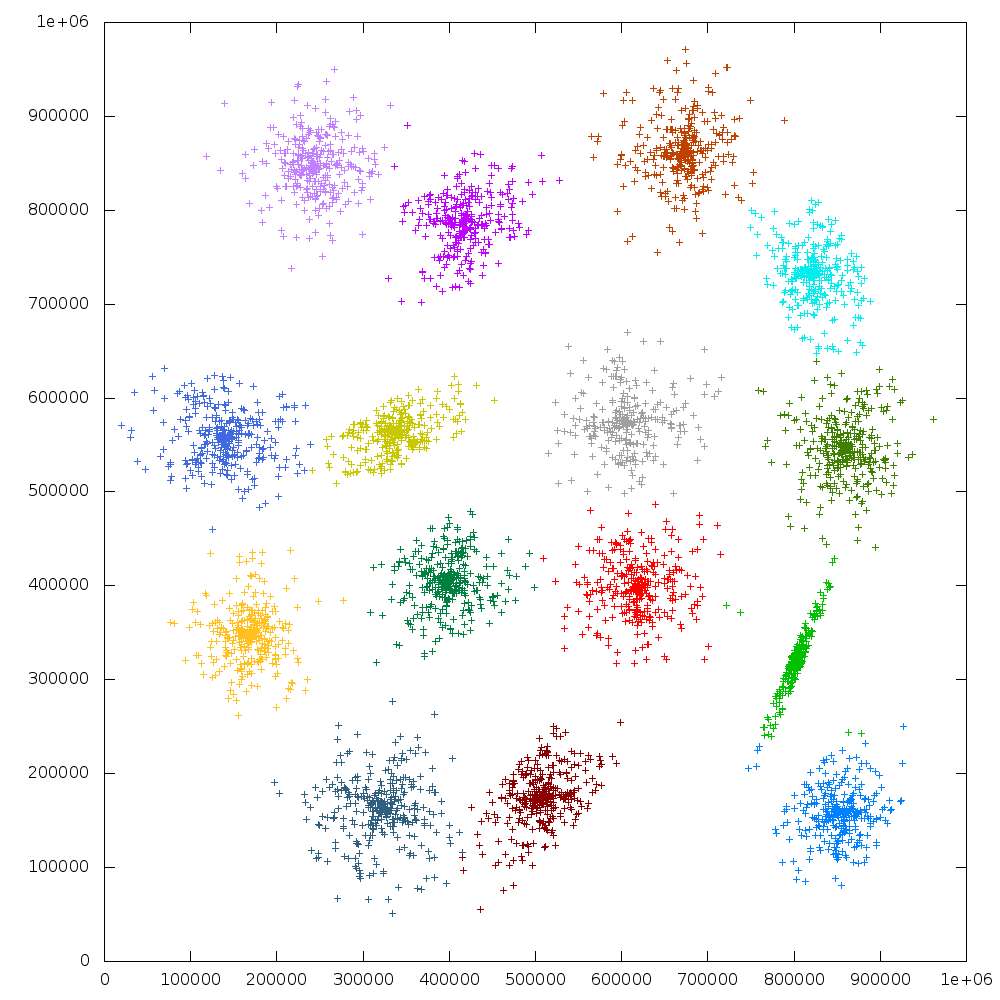
\includegraphics[scale=0.61]{../meanshift/output/pics/s1_colored.png} 
	\vspace{-10pt}
	\caption{Mean Shift S1.txt}
\end{figure}
\section{Algorithmus}
	Für jeden Punkt $ x $ der Eingabe wird ein Verschiebungsvektor $ m $ berechnet. 
		\[ m(x) = \frac{\sum_{x_i \in N(x)} K(x_i - x) x_i }{\sum_{x_i \in N(x)} K(x_i - x)} \]
	Die Punkte $ x_i $ werden in Abhängigkeit der Distanz zu $ x $ gewichtet. Hierfür wird in der Regel ein Gaußkern eingesetzt.
		\[K(x_i - x) = \frac {1}{\sigma\sqrt{2\pi}} e^{-\frac {1}{2} \left(\frac{||x_i - x||}{\sigma}\right)^2}\]
	$ m(x) $ wird nun solange zu $ x $ addiert bis $ x $ konvergiert. Das Clusterzentrum von $ x $ ist genau der Grenzwert von $ x $.[1]\\
	Der Verschiebungsvektor zeigt immer in Richtung der größten Zunahme der Dichte. Im Clusterzentrum ist der Verschiebungsvektor für alle Punkte des Clusters 0.
	Daher existiert genau ein Zentrum pro Cluster.\\
	Da für jeden Punkt unabhängig das Clusterzentrum bestimmt wird, lässt sich der Algorithmus durch Verteilung der zu berechnenden Punkte parallelisieren.\\
\section{Implementation}
	Mean Shift wurde in C implementiert. 
	Eingabe ist ein Menge von Koordinaten. Ausgabe ist eine Liste von Cluster Nummern. Die Visualisierung erfolgt mit Gnuplot.
	Dadurch wird der Code auf das Wesentliche beschränkt.
	Der sequentielle Algorithmus umfasst 100 LOC (Lines Of Code). Die Parallele MPI Version 170 LOC.\\
	Zur Wichtung wird ein Gaußkern genutzt. Dieser muss normiert sein um ein Überspringen eines Clusterzentrums (Verschiebungsvektor $ m = 0 $) zu verhindern.\\
	\vspace{-10pt}
	\begin{figure}[H]
		\centering
		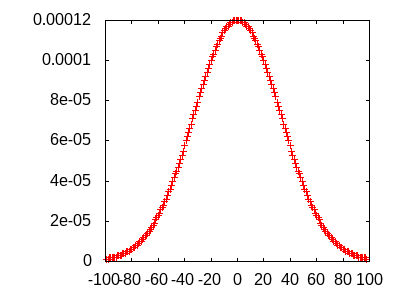
\includegraphics[scale=0.8]{../meanshift/output/pics/gauss.png} 
		\caption{Normierter Gaußkern S1.txt}
	\end{figure}
	Für die Testdaten[2] wurde experimentell eine passende Varianz bestimmt.\\
	Die Punkte werden in einer einfach verketteten Liste gespeichert. Durch Speichern der Punkte in einer Baumstruktur, welche den Ort der
	Punkte berücksichtigt, lässt sich die Implementation noch optimieren. Weit entfernte Punkte könnten so ausgelassen werden.\\
	\subsection{MPI Parallelisierung}
	Beim MPI Mean Shift werden die zu berechnenden Punkte auf die Prozesse gleichverteilt.
	\lstset{language=C,
			basicstyle=\ttfamily,
			keywordstyle=\color{blue}\ttfamily,
			stringstyle=\color{red}\ttfamily,
			commentstyle=\color{green}\ttfamily,
			morecomment=[l][\color{magenta}]{\#}
	}
	\begin{lstlisting}
while(cur_point) {
    if(point_cntr % numprocs == rank)
        cur_point->cluster_nr = do_mean_shift(cur_point->x, cur_point->y);
    cur_point = cur_point->next;
    point_cntr++;
}
	\end{lstlisting}
	Anschließend werden die berechneten Cluster vom Hauptprozess (MPI Prozess mit Rank 0) wieder zusammengeführt und ausgegeben.\\
	Da die Punkte statisch den Rechenknoten zugewiesen werden, ist eine vollständige Auslastung der Cores nicht gewährleistet. 
	Dies könnte durch eine dynamische Verteilung der Punkte optimiert werden. Hier muss überprüft werden, bei welchen Eingaben
	sich der höhere Verwaltungsaufwand lohnt.\\
	Durch Ungenauigkeiten der Fließkommazahlen konvergiert der Verschiebungsvektor $ m(x) $ nicht immmer. Daher muss ein geeignetes $ \delta $
	festgelegt werden, ab welchem, bei Unterschreitung, $ x $ als Clusterzentrum übernommen wird. Bei Testdaten mit Punkten in einem 
	$ 1e + 06 $ großen Quadrat wurde $ \delta = 0.01 $ gewählt. Durch Vergrößern von $ \delta $ kann die Laufzeit des Algorithmus verringert werden.
	Die Anzahl der Fehlklassifikationen steigt jedoch mit $ \delta $ an.\\
	\vspace{-10pt}
	\begin{figure}[H]
		\centering
		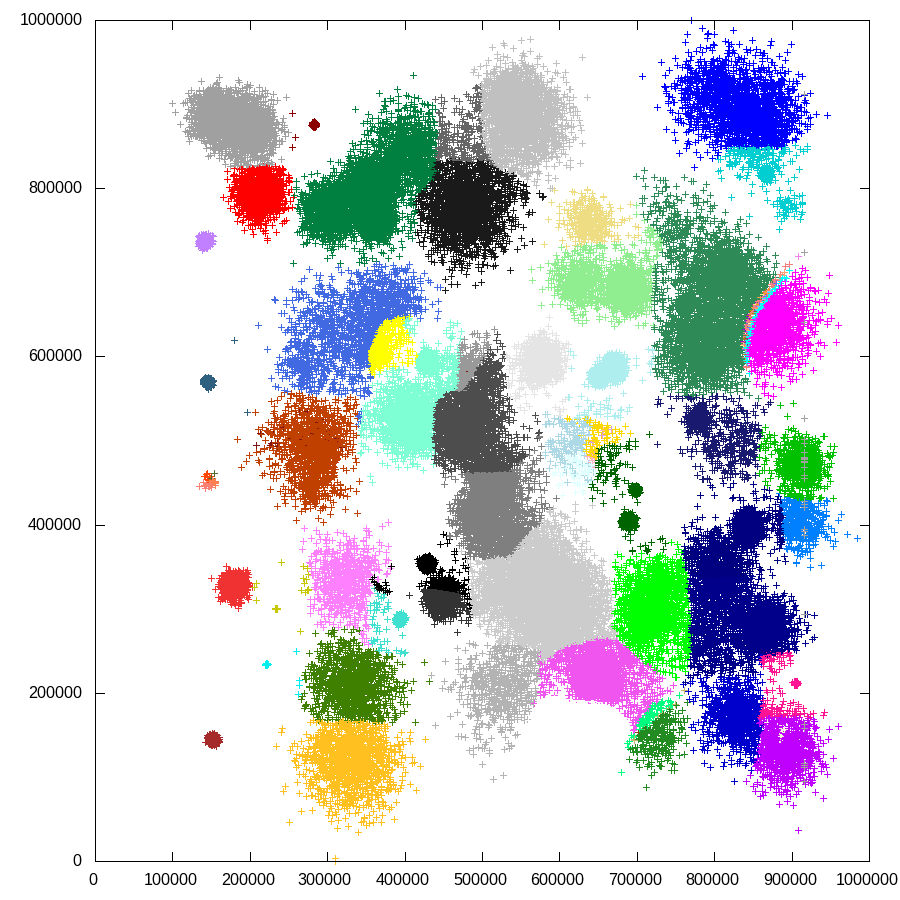
\includegraphics[scale=0.61]{../meanshift/output/pics/birch3_colored.png} 
		\vspace{-5pt}
		\caption{Birch3, 6 Minuten Laufzeit auf 128 Cores}
	\end{figure}
	\newpage
\section{Benchmark}
	Zum Benchmarking wurde die sequentielle und die MPI Version auf dem Hochleistungscluster Taurus[3] gemessen. Mit dem Batchsystem slurm wurden Datensätze mit
	5000 und 100000 Punkten auf 1, 2, 4, 8, 16, 32, 64, 128 und 256 Cores gestartet. Die gemessene Laufzeit des MPI Jobs wird mit der sequentiellen
	Laufzeit verglichen.\\
	\begin{figure}[H] \centering
		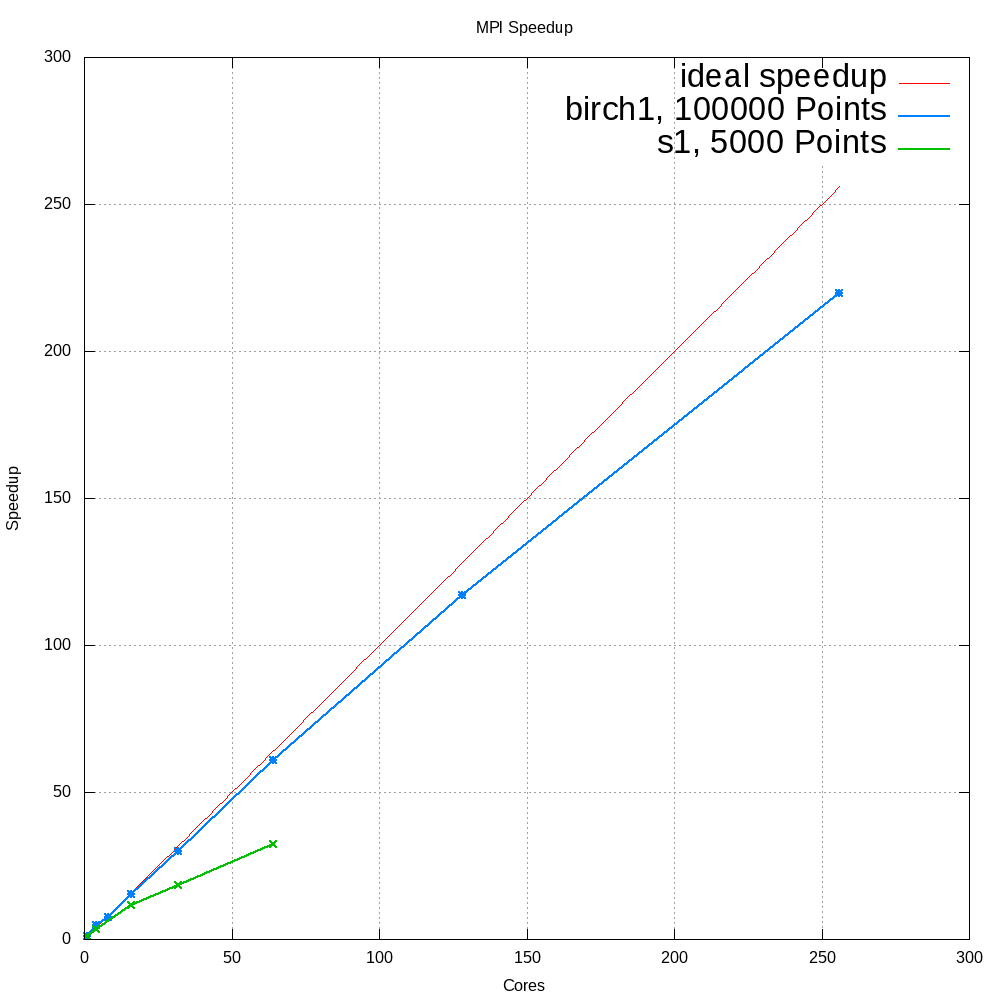
\includegraphics[scale=0.61]{../meanshift/output/pics/speedup.png} 
		\caption{Speedup}
	\end{figure}
	Bei steigender Anzahl an Cores nimmt der Speedup ab. Grund hierfür ist zum größten Teil die statische Verteilung der Punkte und die dadurch
	resultierende nicht optimale Auslastung.\\
	\newpage
	\begin{figure}[H]
		\centering
		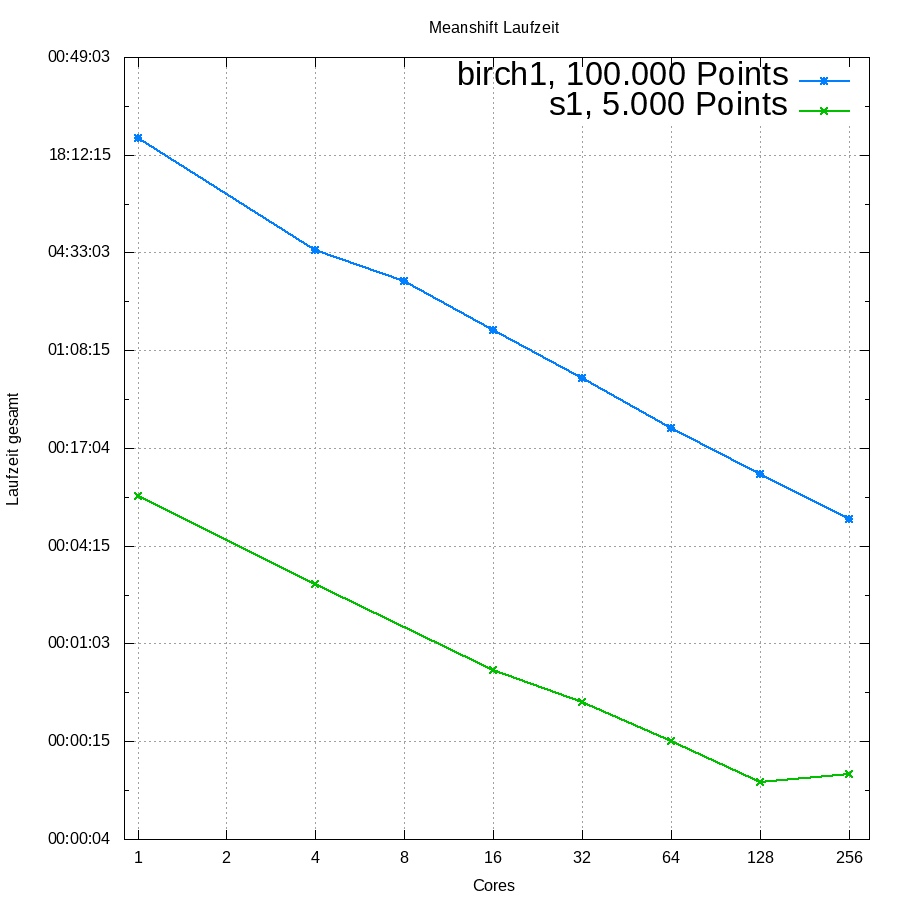
\includegraphics[scale=0.61]{../meanshift/output/pics/benchmark.png} 
		\caption{Laufzeit Benchmark}
	\end{figure}
	Taurus hat jeweils zwei 8 Core Prozessoren auf einem Board. Daher zeigt sich bei 8 und 16 Cores eine Verschlechterung. 
	Ab 16 Cores läuft die Kommunikation zusätzlich über das Netzwerk.\\
	\newpage
\section{Fazit}
	Es existieren viele Möglichkeiten zur Optimierung des parallelen Algorithmus. Zum Beispiel eine dynamische Verteilung der Punkte oder eine dynamische Anpassung
	der Wichtung um die Anzahl der benötigten Mean Shifts zu verringern.\\
	Die Kerngröße muss momentan noch manuell angegeben werden. Dies könnte auch automatisiert werden.\\
	Die markierten Cluster stimmen weitestgehend mit einer intuitiven Markierung überein. Punkte an der Grenze zu zwei Clustern werden jedoch häufig einem 
	dritten Cluster zugeordent (Birch3, (30k,30k)). Hier wäre eine Glättung möglich, um Cluster mit wenigen Punkten in anliegenden Cluster aufzuteilen.\\
	\begin{figure}[H]
		\centering
		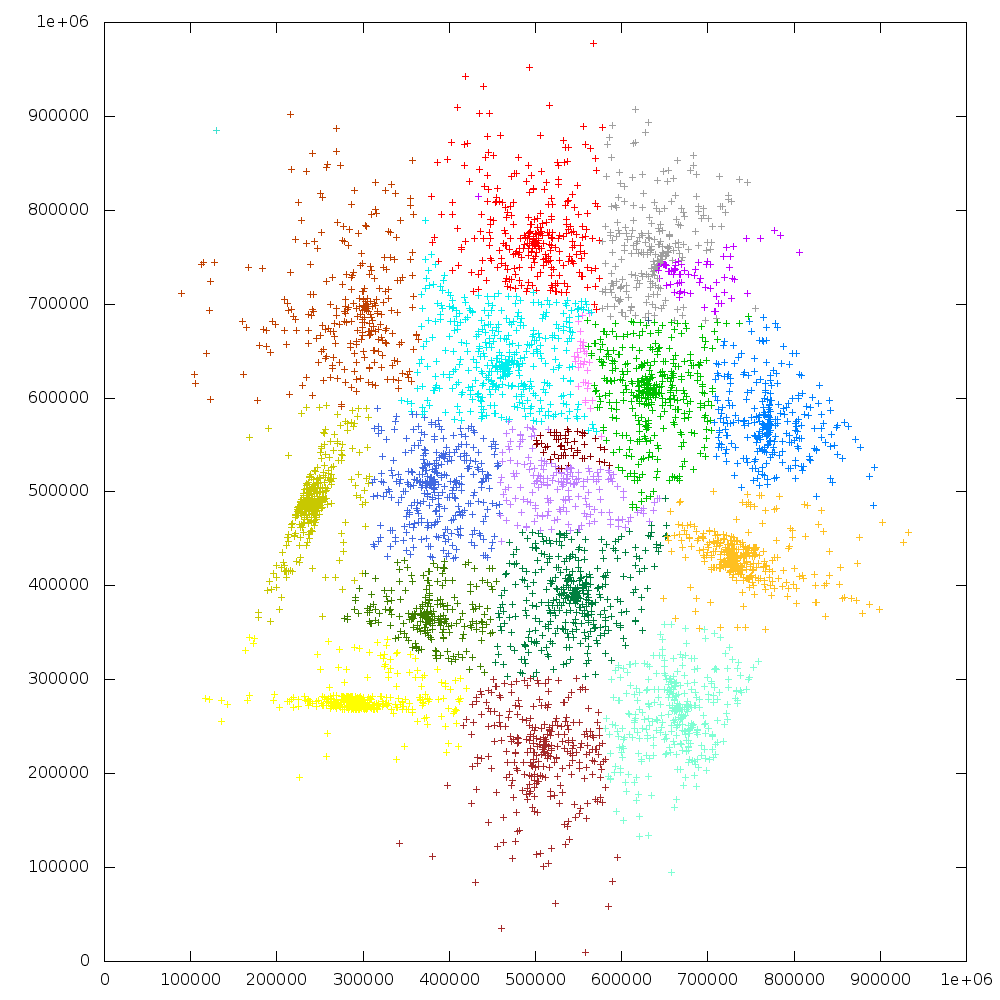
\includegraphics[scale=0.6]{../meanshift/output/pics/s4_colored.png} 
		\caption{S4, 5000 Points}
	\end{figure}
\begin{thebibliography}{999}
	\bibitem [0] {} Meanshift \url{http://homepages.inf.ed.ac.uk/rbf/CVonline/LOCAL_COPIES/TUZEL1/MeanShift.pdf}
	\bibitem [1] {} Mean Shift: Construction and Convergence Proof \url{http://www.cse.yorku.ca/~kosta/CompVis_Notes/mean_shift_derivation.pdf}
	\bibitem [2] {} Datasets \url{http://cs.joensuu.fi/sipu/datasets/}
	\bibitem [3] {} Taurus TU Dresden \url{https://doc.zih.tu-dresden.de/hpc-wiki/bin/view/Compendium/SystemTaurus}
	\bibitem [4] {} Meanshift \url{https://courses.csail.mit.edu/6.869/handouts/PAMIMeanshift.pdf}
	\newline
\end{thebibliography}
